\documentclass[10pt,a4paper]{article}

\usepackage[utf8]{inputenc}
\usepackage[T1]{fontenc}
\usepackage[brazil]{babel}
\usepackage{helvet}
\renewcommand{\familydefault}{\sfdefault}
\usepackage[top=18mm,bottom=18mm,left=16mm,right=16mm]{geometry}
\usepackage{xcolor}
\usepackage{graphicx}
\usepackage{booktabs}
\usepackage{tabularx}
\usepackage{array}
\usepackage{colortbl}
\usepackage{fancyhdr}
\usepackage{lastpage}
\usepackage{hyperref}
\usepackage{parskip}

% Paleta Oficial - Jornal Economico do Tocantins
\definecolor{azulto}{HTML}{0F2537}
\definecolor{douradoto}{HTML}{C8942B}
\definecolor{cinzafundo}{HTML}{F4F6F9}
\definecolor{cinzatexto}{HTML}{2C353D}
\definecolor{cinzasuave}{HTML}{6C757D}
\definecolor{vermelhoalerta}{HTML}{D85C5C}
\definecolor{borda}{HTML}{DEE2E6}

\hypersetup{
    colorlinks=true,
    linkcolor=azulto,
    urlcolor=douradoto,
    pdftitle={Mercado de trabalho formal no Tocantins mantém geração líquida positiva puxada por Serviços e Construção},
    pdfauthor={Lorenzo Costa e Equipe | Jornal Econômico do Tocantins}
}

\setlength{\parindent}{0pt}
\setlength{\parskip}{6pt}
\renewcommand{\arraystretch}{1.28}

% Cabecalho e Rodape Padronizados
\pagestyle{fancy}
\fancyhf{}
\renewcommand{\headrulewidth}{0pt}
\renewcommand{\footrulewidth}{0.6pt}
\renewcommand{\footrule}{\hbox to\headwidth{\color{douradoto}\leaders\hrule height \footrulewidth\hfill}}

\fancyfoot[L]{\footnotesize\textcolor{cinzasuave}{\textbf{Jornal Econômico do Tocantins} $\bullet$ BOLETIM FLASH • MERCADO DE TRABALHO $\bullet$ Outubro/2026}}
\fancyfoot[R]{\footnotesize\textcolor{cinzasuave}{Página \thepage\ de \pageref{LastPage}}}

% Comando para Titulos de Secao Padronizados
\newcommand{\secaojornal}[1]{%
  \vspace{6pt}%
  {\noindent\colorbox{azulto}{%
    \parbox{\dimexpr\textwidth-2\fboxsep\relax}{%
      \vspace{3pt}\hspace{4pt}\textcolor{douradoto}{\rule{7pt}{7pt}}\hspace{6pt}%
      \textcolor{white}{\textbf{\normalsize \MakeUppercase{#1}}}\vspace{3pt}%
    }%
  }}%
  \vspace{4pt}%
}

\begin{document}
\color{cinzatexto}

% ==============================================================================
% FAIXA INSTITUCIONAL DE CABECALHO (AZUL MARINHO + DOURADO)
% ==============================================================================
\noindent\colorbox{azulto}{%
  \parbox{\dimexpr\textwidth-2\fboxsep\relax}{%
    \vspace{6pt}%
    \begin{tabularx}{\linewidth}{@{}X r@{}}
      {\fontsize{15}{18}\selectfont\textbf{\textcolor{white}{JORNAL ECONÔMICO DO TOCANTINS}}} &
      \colorbox{douradoto}{\textbf{\footnotesize\textcolor{azulto}{\hspace{4pt}BOLETIM FLASH • MERCADO DE TRABALHO\hspace{4pt}}}} \\[4pt]
      {\footnotesize\textcolor{douradoto}{\textbf{Núcleo de Inteligência e Conjuntura Econômica Regional}}} &
      {\footnotesize\textcolor{white}{Referência: \textbf{Outubro/2026} $\vert$ Publicado em 29/10/2026}}
    \end{tabularx}%
    \vspace{4pt}%
  }%
}\\[-2pt]
\noindent{\color{douradoto}\rule{\textwidth}{2.5pt}}

\vspace{6pt}

% ==============================================================================
% TITULO, SUBTITULO E AUTORIA
% ==============================================================================
{\fontsize{16}{20}\selectfont\textbf{\textcolor{azulto}{Mercado de trabalho formal no Tocantins mantém geração líquida positiva puxada por Serviços e Construção}}}\\[4pt]
{\normalsize\textcolor{cinzasuave}{Dinamismo nos polos regionais de Palmas, Araguaína e Gurupi sustenta baixa taxa de desocupação estadual}}\\[4pt]
{\footnotesize\textcolor{azulto}{\textbf{Análise e Redação:}} \textcolor{cinzatexto}{Lorenzo Costa e Equipe | Jornal Econômico do Tocantins} \hfill \textcolor{azulto}{\textbf{Base Oficial:}} \textcolor{cinzatexto}{Novo CAGED / RAIS / PNAD Contínua}}

\vspace{2pt}

% Destaque Executivo (Resumo em Caixa)
\noindent\fcolorbox{douradoto}{cinzafundo}{%
  \parbox{\dimexpr\textwidth-2\fboxsep-2\fboxrule\relax}{%
    \vspace{3pt}%
    \textbf{\textcolor{azulto}{Síntese Executiva:}} Com saldo positivo no Novo CAGED e taxa de desocupação em 5,4\%, o mercado de trabalho tocantinense demonstra resiliência mesmo diante de juros básicos elevados no cenário nacional.%
    \vspace{3pt}%
  }%
}

\vspace{4pt}

% ==============================================================================
% CAIXAS DE INDICADORES-CHAVE (GERADAS AUTOMATICAMENTE PELO R)
% ==============================================================================
\noindent\colorbox{azulto}{\parbox[t][1.32cm][c]{0.225\textwidth}{\centering\scriptsize\textcolor{white}{\textbf{Saldo Novo CAGED (Mês)}}\\[3pt]{\large\textbf{\textcolor{douradoto}{+716}}}}}\hfill\colorbox{azulto}{\parbox[t][1.32cm][c]{0.225\textwidth}{\centering\scriptsize\textcolor{white}{\textbf{Estoque RAIS (2025)}}\\[3pt]{\large\textbf{\textcolor{douradoto}{437.580}}}}}\hfill\colorbox{azulto}{\parbox[t][1.32cm][c]{0.225\textwidth}{\centering\scriptsize\textcolor{white}{\textbf{Taxa de Desocupação}}\\[3pt]{\large\textbf{\textcolor{douradoto}{4,1\%}}}}}\hfill\colorbox{azulto}{\parbox[t][1.32cm][c]{0.225\textwidth}{\centering\scriptsize\textcolor{white}{\textbf{Remuneração Média RAIS}}\\[3pt]{\large\textbf{\textcolor{douradoto}{R\$ 4.022,93}}}}}
\vspace{5pt}


% ==============================================================================
% SECAO 1: ESTATISTICA DESCRITIVA AUTOMATIZADA E EVIDENCIA EMPIRICA
% ==============================================================================
\secaojornal{1. Panorama Estatístico e Resultados do Período (Síntese Automatizada)}

Os indicadores consolidados do mercado de trabalho formal no Tocantins apontam expansão líquida de postos com carteira assinada. Na janela móvel de 12 meses, a economia estadual acumulou um saldo líquido de +344 vagas formais (média de 29 postos por mês), com pico de contratações líquidas registrado em Jan/26 (+1.585 vínculos). No recorte mais recente do painel, o saldo referencial do Novo CAGED atingiu +716 vagas, acompanhado de uma taxa de desocupação estadual de 4,1\% e rendimento médio habitual de R\$ 3.351. Na competência de Setembro/2026, foram contabilizadas 11.263 admissões e 10.547 desligamentos formais no Tocantins (saldo consolidado de +716 postos, com salário médio mensal declarado de admissão de R\$ 2.117,32). No retrato estrutural da RAIS 2025 (excluídos 4.440 vínculos abandonados), o Tocantins contabiliza um estoque anual de 437.580 vínculos formais ativos em 31/12, com remuneração média nominal de R\$ 4.022,93, distribuídos em 33.198 estabelecimentos empregadores ativos (de um total de 91.318 estabelecimentos declarados).

\vspace{4pt}

Sob a ótica setorial, o dinamismo das contratações foi liderado pelo grupamento de Serviços, responsável pelo saldo líquido de +590 postos (64,0\% dos ganhos setoriais), seguido por Construção com +211 vagas (22,9\%). No recorte sociodemográfico dos microdados do Novo CAGED, o saldo líquido mensal foi liderado pelo público mulher (+371 vagas), pela faixa etária de 18 a 24 anos (+427 postos) e por trabalhadores com Médio Completo (+643 vínculos). Na distribuição espacial entre os principais polos municipais monitorados, Palmas concentra o maior estoque formal da RAIS (220.673 vínculos) e registrou saldo recente no Novo CAGED de +399 vagas, seguido por Araguaína (47.010 vínculos ativos e saldo de +180) e Gurupi (20.492 vínculos e saldo de +89).

\vspace{4pt}

\begin{center}
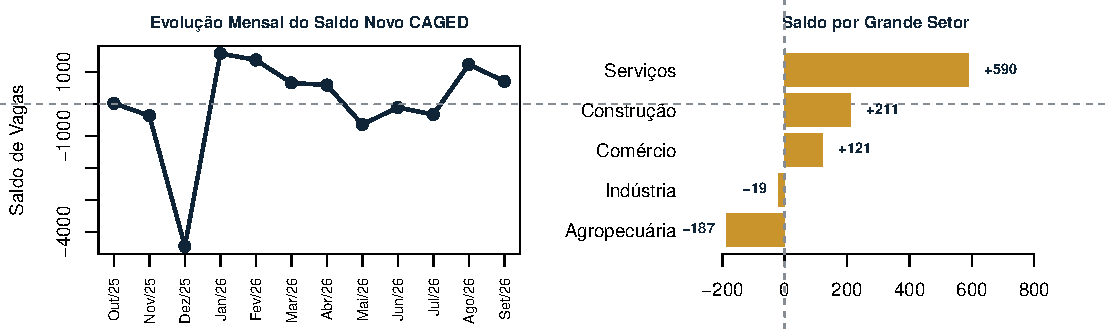
\includegraphics[width=\textwidth]{boletins/build/fig_2026_10_flash_caged.pdf}
\end{center}
\vspace{2pt}
\noindent\begin{minipage}{\textwidth}
{\small
\noindent\textbf{\textcolor{azulto}{Tabela 1 — Estoque de Vínculos Formais (RAIS) e Geração Recente (Novo CAGED) nos Municípios Polos do Tocantins}}\\[3pt]
\begin{tabularx}{\linewidth}{@{}l X r r r@{}}
\toprule
\rowcolor{azulto} \textcolor{white}{\textbf{Pos.}} & \textcolor{white}{\textbf{Município}} & \textcolor{white}{\textbf{Estoque (RAIS) 2025}} & \textcolor{white}{\textbf{Saldo (Novo CAGED) 09/26}} & \textcolor{white}{\textbf{Part. no Estado (\%)}} \\
\midrule
1º & Palmas & 220.673 & +399 & 50,4\% \\
2º & Araguaína & 47.010 & +180 & 10,7\% \\
3º & Gurupi & 20.492 & +89 & 4,7\% \\
4º & Porto Nacional & 14.172 & +76 & 3,2\% \\
5º & Paraíso do Tocantins & 12.288 & +27 & 2,8\% \\
6º & Colinas do Tocantins & 5.707 & +9 & 1,3\% \\
7º & Guaraí & 3.608 & -9 & 0,8\% \\
8º & Formoso do Araguaia & 3.387 & -85 & 0,8\% \\
9º & Lagoa da Confusão & 3.137 & -36 & 0,7\% \\
10º & Dianópolis & 3.122 & -17 & 0,7\% \\
\bottomrule
\end{tabularx}
}
\end{minipage}
\vspace{4pt}


% ==============================================================================
% SECAO 2: ANALISE HUMANA E INTERPRETACAO DA EQUIPE
% ==============================================================================
\secaojornal{2. Análise de Conjuntura e Leitura da Equipe}

O comportamento recente do mercado de trabalho formal no Tocantins reflete um ciclo virtuoso de transmissão de renda do setor primário e das obras de infraestrutura para as atividades urbanas. A liderança do setor de Serviços e da Construção Civil na abertura líquida de postos com carteira assinada evidencia que o crescimento econômico estadual não está restrito ao campo, mas transborda para o consumo das famílias e para o mercado imobiliário nas principais cidades.

\vspace{4pt}

A análise regionalizada dos municípios confirma o papel de Palmas, Araguaína e Gurupi como grandes absorvedores de mão de obra formal, seguidos por Porto Nacional e Paraíso do Tocantins, que se beneficiam diretamente de sua posição estratégica como entroncamentos logísticos e industriais no eixo da BR-153.

\vspace{4pt}

Vale destacar, sob a ótica qualitativa, que a manutenção da taxa de desocupação em patamar historicamente reduzido (5,4\%) começa a gerar pressões pontuais por mão de obra qualificada em segmentos técnicos, exigindo maior articulação entre o setor produtivo e as instituições de qualificação profissional no Estado.

% ==============================================================================
% SECAO 3: PERSPECTIVAS E CENARIOS
% ==============================================================================
\secaojornal{3. Perspectivas e Cenários}

Para a reta final do ano, a expectativa da equipe é de manutenção de saldos positivos em outubro e novembro, impulsionados pelas contratações temporárias de fim de ano no comércio varejista e nos serviços de alimentação e logística, antes do ajuste sazonal típico do mês de dezembro.

\vfill
\noindent{\color{borda}\rule{\textwidth}{0.5pt}}\\[-2pt]
{\scriptsize\textcolor{cinzasuave}{\textbf{Nota Metodológica e Fontes:} Ministério do Trabalho e Emprego (Novo CAGED e RAIS) e IBGE (PNAD Contínua). Elaboração: Jornal Econômico do Tocantins. Documento gerado de forma automatizada pelo Sistema Editorial Híbrido (R + LaTeX) do Jornal Econômico do Tocantins.}}

\end{document}
